% CoDIT 2027 IEEE conference conversion of viXra:2611.0038.
% Research claims follow the authors' empirical preprint. See SOURCE_PROVENANCE.md.
\newif\ifanonymous
\anonymousfalse
\ifdefined\REVIEWVERSION\anonymoustrue\fi
\documentclass[10pt,conference]{IEEEtran}
\IEEEoverridecommandlockouts
\usepackage[T1]{fontenc}
\usepackage[utf8]{inputenc}
\usepackage{cite}
\usepackage{amsmath,amssymb}
\usepackage{booktabs,array}
\usepackage{graphicx}
\usepackage{xcolor}
\usepackage{tikz}
\usepackage{hyperref}
\usepackage{orcidlink}
\usepackage{microtype}
\definecolor{knowInk}{HTML}{0072B2}
\definecolor{adoptInk}{HTML}{D55E00}
\hypersetup{
 colorlinks=true,linkcolor=blue!55!black,citecolor=blue!55!black,urlcolor=blue!55!black,
 pdftitle={The Knowledge Lifecycle of Large Language Models},
 pdfauthor={Amey Thakur; Sarvesh Talele},
 pdfsubject={CoDIT 2027 conference submission},
 pdfkeywords={Knowledge conflict, retrieval-augmented generation, language models, evaluation methodology}
}
\title{The Knowledge Lifecycle of Large Language Models}
\ifanonymous
  \hypersetup{pdfauthor={}}
  \author{\IEEEauthorblockN{Anonymous Submission}}
\else
  \author{
  \IEEEauthorblockN{Amey Thakur\orcidlink{0000-0001-5644-1575}}
  \IEEEauthorblockA{Independent Researcher\\
  Toronto, Canada\\
  \href{https://orcid.org/0000-0001-5644-1575}{ORCID: 0000-0001-5644-1575}\\
  \href{mailto:ameythakur20@gmail.com}{ameythakur20@gmail.com}}
  \and
  \IEEEauthorblockN{Sarvesh Talele\orcidlink{0009-0002-0818-461X}}
  \IEEEauthorblockA{Independent Researcher\\
  Mumbai, India\\
  \href{https://orcid.org/0009-0002-0818-461X}{ORCID: 0009-0002-0818-461X}\\
  \href{mailto:talelesarvesh@gmail.com}{talelesarvesh@gmail.com}}
  }
\fi
\begin{document}
\maketitle
\begin{abstract}
A retrieval-augmented system succeeds only when the document it supplies beats what the model already believes. We measure which one wins, at the level of the token the model would actually emit, over 864 forward passes: six open models from 124M to 1.5B parameters, 24 counterfactual probes, three phrasings, with and without a contradicting document. Restricting to the 304 cases where the model demonstrably held the fact beforehand, the document is adopted 66.8\% of the time and the model keeps its own answer 27.3\%. Which model defers is not predicted by size. Holding the fact rises monotonically with parameter count, from 25.0\% to 98.6\%, but adoption does not: TinyLlama-1.1B holds the fact 97.2\% of the time and still adopts the document least of the six, at 38.6\%, while Qwen2.5-0.5B, less than half its size, adopts 91.8\%. Wording moves the result nearly as much as the model does: over all probes the rate spreads by a median of 47.9 percentage points across three paraphrases, and restricted to conflicts, where the spread measures deference rather than recall, it still reaches 57.6. We also show why this has to be read at the rank: the in-context answer carries more than 0.10 of the probability mass in 332 conditions and is still not what the model says in 69 of them, 20.8\%. That gap is not hypothetical. It is how an earlier version of this work reached a published conclusion that the measurement did not support, which we correct here. All code, probes and measurements are public.
\end{abstract}
\begin{IEEEkeywords}
Knowledge conflict, retrieval-augmented generation, large language models, factual probing, evaluation methodology
\end{IEEEkeywords}
\section{Introduction}
A retrieval-augmented system puts a document in front of a language model and expects the model to use it. When the document contradicts what the model learned in training, one of the two has to give, and which one gives is the question this paper measures. It is not hypothetical: a clinical assistant reading a withdrawal notice, or a coding assistant reading a deprecation note, is useful only if the document wins.

The measurement is easy to get wrong, and we got it wrong. An earlier version of this work concluded that models resist a corrective document, on the strength of the probability the model assigned to the expected answer. That quantity can be small while the model would nonetheless answer correctly, because the mass is spread over a vocabulary of tens of thousands of tokens and the expected answer needs only to be ranked first, not to be large. Re-running the same probes with the rank recorded showed the conclusion did not hold (Section~\ref{sec:correction}). This paper reports the measurement done properly, and the size of the gap we fell into is itself one of the results.

Two changes make it proper. First, we record what the model would actually say, the top-ranked continuation, alongside the probability. Second, we use counterfactual probes rather than real-world updates. A real-world update creates a conflict only for a model whose training data predates it, so across models of different vintages the conflict is present for some and absent for others, and a probability-only readout cannot tell those two cases apart. A counterfactual document asserts something every model is confident is false, so the conflict is present by construction for all of them. This is the standard device in the knowledge-conflict literature~\cite{longpre2021entity,xie2024conflicts}.

Our contributions are:
\begin{enumerate}
\item A rank-level measurement of parametric--context conflict over 864 forward passes, reported on the 304 probe--phrasing pairs where the model demonstrably held the fact and a conflict therefore existed.
\item The finding that deference to a document is not a function of scale. Holding the fact rises monotonically with parameter count across the six models; adopting the document does not, and the 1.1B model that holds the fact most reliably defers least.
\item Evidence that the question's wording moves the outcome nearly as much as the choice of model, by up to 57.6 percentage points of deference alone, and a separation of that effect from the larger one the wording has on whether the model holds the fact at all (Section~\ref{sec:phrasing}).
\item Evidence that a probability-only readout cannot support a claim about what a model answers, and a correction of our own earlier report on exactly that ground (Section~\ref{sec:correction}).
\end{enumerate}
Code, probe set and measurements are public~\cite{thakur2026code}.

\section{Method}
\label{sec:method}
\subsection{Probes and phrasings}
Each probe is a country whose capital no model of this size should get wrong, paired with a counterfactual that is a real, prominent city of the same country: France and Lyon, Japan and Osaka, Egypt and Alexandria, and 21 others. Using a real city keeps the substitution plausible rather than nonsensical. Holding the fact type fixed across all 24 probes means that a difference between probes is not a difference between kinds of question. The document asserts the substitution as a constitutional relocation and names the new capital twice.

Each probe is asked three ways, differing in wording but not in what is asked. A quantity that moves across the three is a property of the sentence rather than of the model's knowledge, and reporting the spread is what lets a reader tell those apart.

\subsection{Conditions and models}
Every probe and phrasing is run twice: once with the question alone, which measures what the model believes, and once with the contradicting document prepended, which measures what it does about the conflict. The first condition is not a control in name only. It is what identifies the subset in which a conflict exists at all, and every headline number in this paper is restricted to that subset.

Six open models span an order of magnitude: GPT-2 at 124M, 355M and 774M~\cite{radford2019gpt2}, Qwen2.5-0.5B-Instruct and Qwen2.5-1.5B-Instruct~\cite{yang2024qwen2}, and TinyLlama-1.1B-Chat~\cite{zhang2024tinyllama}. All run in float32 on CPU, so the numbers reproduce on ordinary hardware rather than depending on a particular accelerator's arithmetic.

\subsection{Recorded quantities}
For a prompt $x$ the model defines a distribution $p_\theta(\cdot \mid x)$ over the vocabulary. Writing $t$ for the first token of the true answer and $c$ for the first token of the counterfactual, we record $p_\theta(t \mid x)$ and $p_\theta(c \mid x)$, the rank of each, and $\arg\max_v p_\theta(v \mid x)$. Rank determines the answer under greedy decoding; probability is what the earlier report used alone.

That distribution is the softmax over the final layer's output, the standard construction for a transformer decoder~\cite{vaswani2017attention}, and we follow the usual account of the feed-forward blocks and the softmax that turns their output into a distribution~\cite{thakur2021fundamentals}. One consequence of training by maximum likelihood matters here: such a model spreads mass over everything the context makes plausible rather than committing to a single continuation, unlike a generator trained against a discriminator~\cite{thakur2021gan}. That is precisely why a modest probability does not mean the token is not the answer, and it is the mechanism behind the gap reported in Section~\ref{sec:rank}.

Answers are compared at the first token. Tokeniser boundaries were checked for every probe, phrasing and model: all 144 country--answer pairs tokenise cleanly across the three tokeniser families used here, so no probe silently measures a merged token.

\section{Results}
Table~\ref{tab:results} reports all six models, and Fig.~\ref{fig:scale} draws the two columns the paper turns on.

\begin{table}[t]
\caption{Model behaviour when a document contradicts a known fact.}
\label{tab:results}
\centering
\footnotesize
\setlength{\tabcolsep}{3pt}
\begin{tabular}{@{}lrrrrrr@{}}
\toprule
Model & Params & Knows & $n$ & Adopts & Keeps & Spread\\
 & (M) & (\%) & & (\%) & (\%) & (pp)\\
\midrule
GPT-2 & 124 & 25.0 & 18 & 50.0 & 16.7 & 62.5\\
GPT-2 medium & 355 & 54.2 & 39 & 43.6 & 56.4 & 41.7\\
GPT-2 large & 774 & 79.2 & 57 & 75.4 & 24.6 & 29.2\\
Qwen2.5-0.5B-Instruct & 494 & 68.1 & 49 & 91.8 & 8.2 & 87.5\\
TinyLlama-1.1B-Chat & 1100 & 97.2 & 70 & 38.6 & 57.1 & 54.2\\
Qwen2.5-1.5B-Instruct & 1540 & 98.6 & 71 & 87.3 & 0.0 & 37.5\\
\bottomrule
\end{tabular}
\par\smallskip
\parbox{\columnwidth}{\scriptsize
\emph{Knows} is the percentage of 72 probe--phrasing pairs where the true answer is top-ranked without the document. The remaining columns are restricted to the $n$ cases where that held. \emph{Adopts} and \emph{Keeps} are percentages of the counterfactual and true answer, respectively, being top-ranked with the document; they need not sum to 100 because a third token may rank first. \emph{Spread} is the range across three wordings of the counterfactual top-rank rate over all 24 probes, not restricted to conflicts.
}
\end{table}

\begin{figure}[t]
\centering
\resizebox{\columnwidth}{!}{%
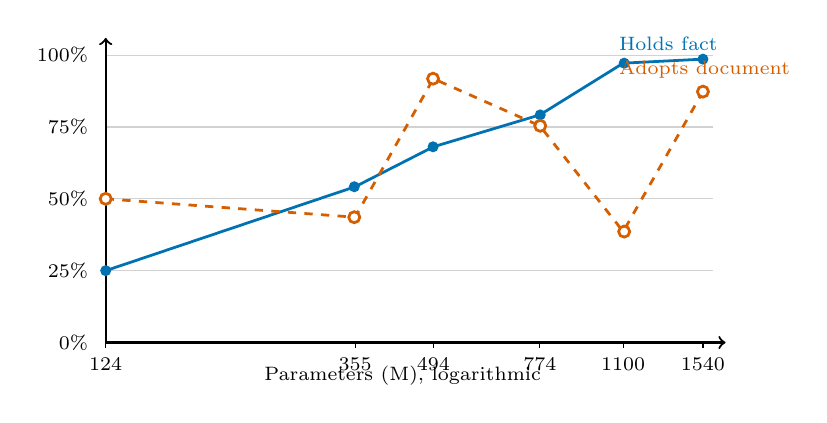
\begin{tikzpicture}[x=0.82cm,y=0.73cm]
\foreach \y/\lab in {0/0,1.25/25,2.5/50,3.75/75,5/100}{
 \draw[gray!35] (0,\y)--(9.4,\y);
 \node[font=\scriptsize,anchor=east] at (-0.12,\y) {\lab\%};
}
\draw[->,thick] (0,0)--(9.6,0);
\draw[->,thick] (0,0)--(0,5.3);
\foreach \x/\lab in {0/124,3.862/355,5.075/494,6.724/774,8.015/1100,9.25/1540}{
 \draw (\x,0)--(\x,-0.1) node[below,font=\scriptsize]{\lab};
}
\draw[line width=1pt,knowInk] (0,1.25)--(3.862,2.71)--(5.075,3.405)--(6.724,3.96)--(8.015,4.86)--(9.25,4.93);
\foreach \x/\y in {0/1.25,3.85/2.71,5.07/3.405,6.73/3.96,8.03/4.86,9.25/4.93}{
 \fill[knowInk] (\x,\y) circle (2pt);
}
\draw[line width=1pt,adoptInk,dashed] (0,2.5)--(3.862,2.18)--(5.075,4.59)--(6.724,3.77)--(8.015,1.93)--(9.25,4.365);
\foreach \x/\y in {0/2.5,3.85/2.18,5.07/4.59,6.73/3.77,8.03/1.93,9.25/4.365}{
 \draw[adoptInk,fill=white,line width=1pt] (\x,\y) circle (2pt);
}
\node[font=\scriptsize,knowInk,anchor=west] at (7.8,5.2) {Holds fact};
\node[font=\scriptsize,adoptInk,anchor=west] at (7.8,4.75) {Adopts document};
\node[font=\scriptsize] at (4.6,-0.58) {Parameters (M), logarithmic};
\end{tikzpicture}%
}
\caption{Holding a fact scales with parameter count; deferring to a contradictory document does not. Filled markers show the true answer top-ranked without a document; open markers show the document answer top-ranked over genuine conflicts.}
\label{fig:scale}
\end{figure}

\subsection{Holding a fact scales; deferring to a document does not}
Whether a model holds the fact at all rises monotonically with parameter count, from 25.0\% at 124M to 98.6\% at 1.5B, with no inversion anywhere in the ordering. This is the expected result and serves mainly as a check that the probes measure what they are meant to.

What the model then does with a contradicting document follows no such pattern. Across the 304 genuine conflicts the document is adopted 66.8\% of the time and the model keeps its own answer 27.3\%, but the per-model rates run from 38.6\% to 91.8\% in an order that has little to do with size. The clearest case is TinyLlama-1.1B: it holds the fact 97.2\% of the time, the second-highest of the six, and yet adopts the document in only 38.6\% of its 70 conflicts, keeping its own answer in 57.1\%. Qwen2.5-0.5B, less than half its size, adopts 91.8\%. The two Qwen models, at 494M and 1540M, are the two most deferential; the three GPT-2 models and TinyLlama are not ordered by size among themselves.

The natural reading is that deference is a property of how a model was trained rather than of how large it is. We cannot separate those factors here: the six models differ in family, in instruction tuning and in scale at once, and the design does not let us hold two fixed while varying the third. What the data do establish is the negative claim: scale alone does not buy a model that uses the document in front of it. Qwen2.5-1.5B is the only model in the set that never keeps its own answer once contradicted, at 0.0\%.

\subsection{Wording moves the answer, and moves two things at once}
\label{sec:phrasing}
How the question is worded changes the outcome substantially, and separating what it changes is worth doing, because the two mechanisms carry different advice.

The coarse quantity is the rate at which the counterfactual is top-ranked over all 24 probes of a wording, with no restriction to conflicts. Across the three wordings it has a median spread of 47.9 percentage points and a maximum of 87.5, and that maximum is Qwen2.5-0.5B, which ranks the counterfactual first 100.0\% of the time under its most favourable wording and 12.5\% under its least.

That figure is not a measure of deference. Under its third wording Qwen2.5-0.5B holds the fact in 1 of its 24 probes rather than in all 24, so there is almost no conflict left for it to resolve; in the single conflict that remains it does adopt the document. Restricted to conflicts, its adoption rate across the three wordings is 16.7 points wide, not 87.5. Most of what the wording moved was whether the model knew the fact, not whether it deferred.

Deference does move, and by less. The adoption spread is defined only for the 4 models whose every wording leaves at least one conflict, and over those it has a median of 35.1 percentage points and a maximum of 57.6. The maximum is TinyLlama-1.1B, which adopts the document 17.4\% of the time under one wording and 75.0\% under another, on conflicts in every case.

A spread of 57.6 points in deference alone is larger than the gap between most pairs of models in Table~\ref{tab:results}. A single-phrasing result about knowledge conflict reports a property of the sentence at least as much as a property of the model. It also has to say which rate it is reporting, since the two differ here by a factor of five on the same model.

\subsection{Probability is not an answer}
\label{sec:rank}
The in-context answer carries more than 0.10 of the probability mass in 332 of the 432 conditions with the document present, and in 69 of those, 20.8\%, it is still not the token the model ranks first. A reader given only the probability would conclude the document had landed; a reader given the rank would see that the model would say something else.

The converse also holds. A small probability for the expected answer is compatible with that answer being ranked first, because the mass is distributed over a large vocabulary. Neither direction of inference from probability to answer is safe. Recording the rank costs one comparison against the maximum, and it is the only quantity that corresponds to what a system deployed under greedy decoding will actually produce.

\section{A correction to our earlier report}
\label{sec:correction}
An earlier version of this work reported that across six models and three documented fact changes the conflict did not resolve, and that no model answered a drug-withdrawal probe correctly under any of three phrasings. That claim was wrong, and the manner of its wrongness is the reason this paper exists.

The script that produced it recorded, for each model and phrasing, the surprisal of the expected answer with the document present. It recorded neither the rank of that answer nor the identity of the top-ranked token. A claim about what a model answers cannot be derived from that quantity, and when we re-ran the same probes with the rank recorded, three of the six models ranked the corrected answer first under two of the three phrasings.

A second defect was structural. The probes were real-world updates, so whether a model held the superseded fact depended on its training cutoff, and the six cutoffs differ. For the drug probe the event predates every model's training data, so no model held the superseded fact and there was no conflict to resist. The large surprisal we reported was the question frame declining a participle, not a model defending a stale belief. Both defects are removed by the design in Section~\ref{sec:method}: counterfactual probes make the conflict independent of cutoff, and the no-document condition identifies the cases where the model actually held the fact.

We report this at length because the correction generalises. A probability-only readout is cheap to compute and easy to tabulate, and it will return a number for any probe whether or not that probe tests anything at all. Both defects would have been caught immediately by recording the rank, which is one comparison.

\section{Related work}
Factual probing of language models has used the top-ranked continuation as its readout since Petroni et al.~\cite{petroni2019lama} posed the question. Min et al.~\cite{min2022rethinking} make the general point for in-context learning, where the quantity a prompt moves is not the quantity the model acts on. Jiang et al.~\cite{jiang2020know} show that the prompt used to query a model changes how much knowledge is extracted from it. Elazar et al.~\cite{elazar2021consistency} measure consistency over paraphrases and find pretrained models frequently inconsistent under paraphrase.

The expectation that capability improves with parameter count is the default reading of scaling literature~\cite{kaplan2020scaling,hoffmann2022chinchilla}. Instruction tuning optimises models to follow what they are given~\cite{ouyang2022instructgpt,wei2022flan}; separating family, tuning and scale requires a design that holds two of the three fixed.

Supplying a document does not guarantee the model uses it. Liu et al.~\cite{liu2024lost} show retrieved evidence is used unevenly depending on context position, and Chen et al.~\cite{chen2024benchmarking} evaluate how systems respond to counterfactual passages. Longpre et al.~\cite{longpre2021entity} construct conflicts by substituting entities in retrieved passages. Xie et al.~\cite{xie2024conflicts} report that receptiveness depends on evidence coherence. Du et al.~\cite{du2024context} quantify how context moves a model's answer distribution, and Xu et al.~\cite{xu2024conflicts} survey knowledge conflicts.

Retrieval is standard practice~\cite{lewis2020rag,guu2020realm,gao2023ragsurvey}; editing parametric memory directly~\cite{meng2022rome,meng2023memit} does not remove possible disagreement between weights and context at inference. Transformer feed-forward layers can function as key-value memories~\cite{geva2021kv}. The synchronization framing relates parametric memory and retrieved context to replicas of a fact, where resolution needs an explicit protocol~\cite{thakur2022clock}.

\section{Limitations}
The models are small. The largest is 1.5B parameters, and behaviour at 7B and above may differ. The design confounds family, instruction tuning and scale. We can show that adoption is not ordered by parameter count, but cannot attribute the variation to any one factor.

The probes are homogeneous by construction. Every one is a national capital, which controls for question type at the cost of telling us nothing about numeric, temporal or causal facts. Counterfactual probes remove the cutoff confound but the document asserts something false. A deployed retrieval system meets the opposite case, where the document is true and parametric memory is stale. A model that looks deferential here may also be deferential to misinformation.

Answers are compared at the first token, sufficient here because candidate cities differ there, but not general. The measurement is a single-turn next-token distribution under greedy reading; systems that sample, reason over several steps, or are prompted to weigh sources explicitly may behave differently.

\section{Conclusion}
Across 304 genuine conflicts in six open models, a contradicting document is adopted 66.8\% of the time. Whether a given model adopts it is not predicted by size: holding the fact rises monotonically with parameter count while deference does not, and the model that holds facts second-most reliably defers least of all. The wording of the question moves the rate by up to 87.5 percentage points, comparable to the spread between models.

The methodological result is that the probability a model assigns to an answer and the answer it gives are different quantities. They disagree in 20.8\% of the measured conditions, and an earlier published conclusion rested on the difference. Rank is one comparison more expensive and is what a deployed system actually emits.

\section*{Future work}
A natural extension is multimodal. When contradicting evidence is an image rather than a passage, the same question arises with no token rank to read the answer from. Image translation~\cite{thakur2021whitebox,thakur2021aoda} and zero-shot visual detection~\cite{thakur2026accident}, where a model must lean on parametric knowledge because no corrective document exists, are settings where this diagnostic is missing. A second direction is deployment: the accompanying demonstration runs a model in the browser~\cite{thakur2026demo}; a conflict diagnostic cheap enough to run there would put the measurement where retrieval happens.

\section*{Code and data availability}
Code, probe set and measurements are publicly available in the authors' repository~\cite{thakur2026code}. The cross-model sweep is also published as a notebook~\cite{thakur2026notebook}, and an interactive demonstration runs in the browser~\cite{thakur2026demo}.

\bibliographystyle{IEEEtran}
\ifanonymous
  \bibliography{references-review}
\else
  \bibliography{references}
\fi
\end{document}
